\documentclass[10pt,twocolumn,letterpaper]{article}
\usepackage[margin=0.72in,columnsep=0.26in]{geometry}
\usepackage[T1]{fontenc}
\usepackage{times,microtype,amsmath,amssymb,booktabs,graphicx,tikz,array}
\usetikzlibrary{arrows.meta,positioning,fit}
\usepackage[breaklinks,colorlinks,urlcolor=blue,citecolor=black,linkcolor=black]{hyperref}
\usepackage{url,balance}
\raggedbottom
\setlength{\parindent}{1em}
\setlength{\parskip}{0pt}
\newcommand{\artifact}[2]{\href{https://github.com/rz4/reticuli/blob/5318acaac34ef99eeba9ff064a995a6313cc70ec/#1}{#2}}
\title{Self-Hosting Software Reconstruction\\from Executable Specifications}
\author{Rafael Zamora-Resendiz}
\date{Working manuscript --- October 12, 2026}
\begin{document}
\maketitle
\begin{abstract}
Can a software system be rebuilt from its acceptance criteria alone? And can the rebuilt system then do the same job on itself? We present a method for studying those two questions. It rests on three elements: executable specifications, identifiers that do not depend on the implementation, and reconstruction repeated across generations.

The method keeps the specification separate from generated source. It builds each component on dependencies that were themselves reconstructed. And it evaluates every result twice --- once as a candidate implementation, once as the tool that must produce the next one. The second evaluation is what exposes requirements ordinary conformance tests leave implicit, including the assumptions the evaluator itself makes. We separate three claims that are easily conflated: successful reconstruction, operational self-hosting, and refinement of the specification. Each needs different evidence, and we say what.

Reticuli is the prototype and the case study. Its archived campaign records reconstructions from two model families that pass the system criteria, and a complete second-generation implementation built under a reconstructed kernel. Two supporting experiments, on a parser and on jq, show how reconstruction surfaces missing obligations and the weakness of example-only specifications. Together these establish a finite, test-relative instance of self-hosting reconstruction --- and identify what remains: the bootstrap dependencies still in place, and validation by an operator outside our environment.
\end{abstract}

\section{Introduction}
A software system is usually preserved through its source code and the toolchain that builds it. An alternative is to preserve an executable description of what it must do, then construct a new implementation that satisfies that description. The two approaches preserve different things: a build reproduces an implementation, whereas reconstruction attempts to recover required behavior while allowing the implementation to change.

Code-generating models make this distinction experimentally accessible. Given tests, interface definitions, fixtures, and dependency contracts, a producer can attempt to write a replacement without receiving the original source. The outcome is informative in either direction. Success demonstrates that the supplied material supports at least one accepted realization. Failure can expose a limitation of the producer, an omitted requirement, an environmental dependency, or a defect in the evaluation procedure. Determining which explanation applies is part of the method.

The problem becomes recursive when the target is the reconstruction system itself. A replacement must then do more than satisfy its own test suite. It must construct workspaces, invoke producers, execute criteria, preserve specification identity, and produce another usable reconstruction. This makes self-hosting a demanding integration experiment: assumptions hidden inside the construction and evaluation machinery become requirements of the system being reconstructed.

We study the following question: \emph{under what operational conditions can an executable specification support successive reconstruction of the system that interprets it?} The contribution is a method for running and reading that experiment. It has four parts. A representation separates specification identity from implementation bytes. Reconstruction proceeds in layers, each built on already reconstructed dependencies. The result is then evaluated twice: once as an object, once as the tool doing the work. Finally, discovered omissions become versioned changes to the specification rather than silent adjustments.

This paper hedges often, and on purpose. So we state the scope once, in plain terms.

\vspace{2pt}\noindent\textbf{What the case study shows.} One specification identity stayed fixed throughout. Two model families generated implementations that passed its system criteria. A generated tool then sealed inputs, confined gates, and orchestrated the construction of a complete successor. That successor reconstructed a component through its own interface. Replacement also exposed requirements the component criteria had left implicit. On an external target, one signed refinement measurably reduced one producer family's divergence.

\vspace{2pt}\noindent\textbf{What it does not show.} Five things, each marked wherever it bears on a claim. The criteria do not characterize the software's behavior. The producers may fail alike. The chain is not shown to continue past the generations observed. We cannot verify that a producer never saw the original. And no operator outside our own environment has repeated the judgment; that condition is open.

Reticuli serves as the prototype and empirical case study~\cite{repo}. Sections~\ref{sec:specs} and~\ref{sec:method} develop the representation and the method. Section~\ref{sec:obligations} covers the refinement loop and the discipline that keeps it honest. Section~\ref{sec:empirical} reports the campaign, claim by claim.

\section{Executable specifications as reconstruction targets}
\label{sec:specs}
\subsection{What is preserved?}
An executable specification $S$ consists of a recipe, required interfaces, acceptance programs, fixtures, and other declared inputs. An implementation $I$ contains the replaceable source or generated artifacts. The distinction is operational: the experiment declares which bytes constrain acceptance and which bytes the producer must reconstruct.

Concretely, in the prototype a specification is a directory: a recipe naming each file's role, a set of executable acceptance programs, their fixtures, and the pinned outputs those programs must produce. The implementation is whatever source satisfies them. A producer is handed a copy of that directory with the implementation files absent --- the recipe still declares that they must exist and what their acceptance program expects --- and writes them. The acceptance programs then run against what it wrote. Nothing in this arrangement requires a model: the same directory can be handed to a person.

Let $e$ denote the execution environment, $b$ the resource envelope, and $z$ the seed of any randomized checks. Write
\begin{equation}
 A(S,I;e,b,z)\in\{\mathrm{pass},\mathrm{fail},\mathrm{unknown}\}.
\end{equation}
The third outcome distinguishes missing or inconclusive evidence from rejection by the specification. An explicitly specified timeout may count as failure; an unavailable execution platform may instead make the experiment inconclusive. The reporting policy must be fixed in advance.

For fixed evaluation conditions, the specification admits a set
\begin{equation}
 \mathcal{I}_S=\{I:A(S,I;e,b,z)=\mathrm{pass}\}.
\end{equation}
Membership is weaker than behavioral equivalence. Two members may disagree on any input the criteria do not exercise, and a different seed or environment may change a verdict. So the useful question is not whether the tests determine every behavior. It is whether the admitted implementations preserve the behavior some particular use needs.

\subsection{Stable identity across changing implementations}
To compare generations, the specification needs an identity that does not depend on the generated implementation. A general construction is
\begin{equation}
 \rho(S)=H\!\left(\operatorname{canon}(\text{recipe},\{p,H(B_p)\})\right),
\end{equation}
where $B_p$ is the content of each declared specification file at path $p$, and $H$ is a cryptographic hash. Generated implementation bytes are omitted. The exact canonical representation is a protocol choice and must itself be specified and tested.

This identifier answers whether two runs used the same committed specification. It does not determine whether their implementations pass. Identity checking and execution of the acceptance criteria are therefore separate operations. Nor does it identify mathematical semantics: two differently written specifications can admit the same behavior while receiving different identifiers.

Construction hints need care. Suppose a hint sits outside the identity but the acceptance program can read it. Then changing the hint changes the verdict without changing the identifier. Two fixes are available: commit the hint along with the rest, or stop the evaluator from reading it. Either way, separating construction context from judgment context is an enforceable requirement, not a documentation convention.

\subsection{Reconstruction and replaceability}
A producer $P$ proposes implementations from the permitted view $V(S)$ of the specification. A reconstruction tool $T$ materializes that view, invokes $P$, and evaluates candidates:
\begin{equation}
 R_T(S,P;e,b)\longrightarrow (I,\tau)\ \text{or a refusal},
\end{equation}
where $\tau$ records the relevant inputs, attempts, verdicts, and generated artifact digests. The producer may be a model, a synthesis procedure, or a human. The method does not require one particular generator.

For a consumer $C$, let $Q(C[I])$ express the required downstream behavior. A specification is sufficient for that consumer only if every admitted implementation preserves $Q$. Reconstruction provides a way to search for counterexamples:
\begin{equation}
 I\in\mathcal{I}_S\quad\text{and}\quad Q(C[I])=\mathrm{false}.
\end{equation}
Such a witness identifies a mismatch between the acceptance criteria and the consumer's requirements. Finding many successful substitutions increases empirical confidence but cannot establish the universal condition for unrestricted programs.

\section{A method for self-hosting reconstruction}
\label{sec:method}
\subsection{Define the bootstrap boundary}
Self-hosting requires a precise account of what reproduces itself. The reconstruction tool, producer, runtime, operating system, acceptance programs, and experiment driver are distinct components. A reconstructed orchestration kernel does not imply that the model, interpreter, or host platform was reconstructed.

Before the experiment, partition the system into three parts: the implementation to replace, the specification that remains fixed, and the external infrastructure that remains available. Record which components may execute during construction and which may appear in the producer's workspace. Source exclusion from a workspace is a testable access condition; absence of prior exposure in a model's training data is a different and usually unverified claim.

This explicit partition permits partial but meaningful self-hosting. A generated tool can take responsibility for sealing inputs, launching reconstruction, and enforcing gates while relying on an external producer. The report should name these transferred responsibilities rather than describe the entire computing stack as self-reproducing.

\subsection{Reconstruct in dependency order}
A monolithic reconstruction can obscure whether failure came from local functionality, integration, or an exhausted generation budget. Decompose the target into a directed acyclic graph of components. Cyclic dependencies can be grouped into a component or broken by an explicitly retained bootstrap interface. Each component has local criteria, a declared interface, and dependencies available during construction.

Reconstruct the components in topological order. For component $v$ in generation $g$, supply already reconstructed dependencies $I_{g,\mathrm{dep}(v)}$ as construction context. Withhold the original implementation of $v$. Once accepted locally, its generated bytes become context for later components in the same generation.

This choice matters because local conformance does not imply compatibility with undocumented private interfaces. Keeping an original upper layer while replacing the layer beneath it can create an accidental requirement to reproduce private names or calling conventions. Constructing the upper layer against the actual reconstructed dependency allows internal organization to vary while the declared external obligations remain fixed.

Intermediate construction specifications may commit to the particular lower-layer bytes supplied to a producer. Their identifiers can therefore differ across lineages. These intermediate specifications are scaffolds; they must not be confused with the identity of the whole target. After assembly, evaluate the complete generated implementation against the original, unchanged system-level specification.

\subsection{Separate local acceptance from system acceptance}
Local gates keep the construction process tractable, but they do not establish that the assembled system works. A system-level evaluation must exercise interactions that component tests may miss: dependency resolution, serialization round trips, artifact transfer, error propagation, and resource use across the complete dependency graph.

The experiment should preserve both outcomes. A component that passes locally but fails after composition is evidence about the decomposition or the strength of its contract. Re-running only the failed unit test loses that evidence. Similarly, changing the system gate to accommodate a candidate creates a new target and must not be counted as successful reconstruction of the previous one.

\subsection{Evaluate the candidate in two roles}
A self-hosting tool has two experimentally distinct roles.

\paragraph{Object role.} An existing evaluator tests the candidate implementation as data or executable content. This establishes whether the candidate passes the fixed specification under that evaluator. For example, a reference harness may substitute the candidate's modules and run the system acceptance suite.

\paragraph{Operator role.} The candidate becomes the tool that performs the work. It must prepare a fresh room, invoke a producer, execute acceptance programs using its own execution layer, manage dependencies, and emit a result whose identity and verdict can be checked externally. A candidate may pass the object-role test yet fail here because its sandbox, subprocess handling, or artifact transport is insufficient.

Both roles require negative controls. Altering a committed criterion should be detected; a known invalid implementation should be rejected; an intact package should remain usable after transport. A tool that accepts its own successor is not persuasive evidence unless the acceptance behavior has also been tested against failures.

\begin{figure*}[t]
\centering
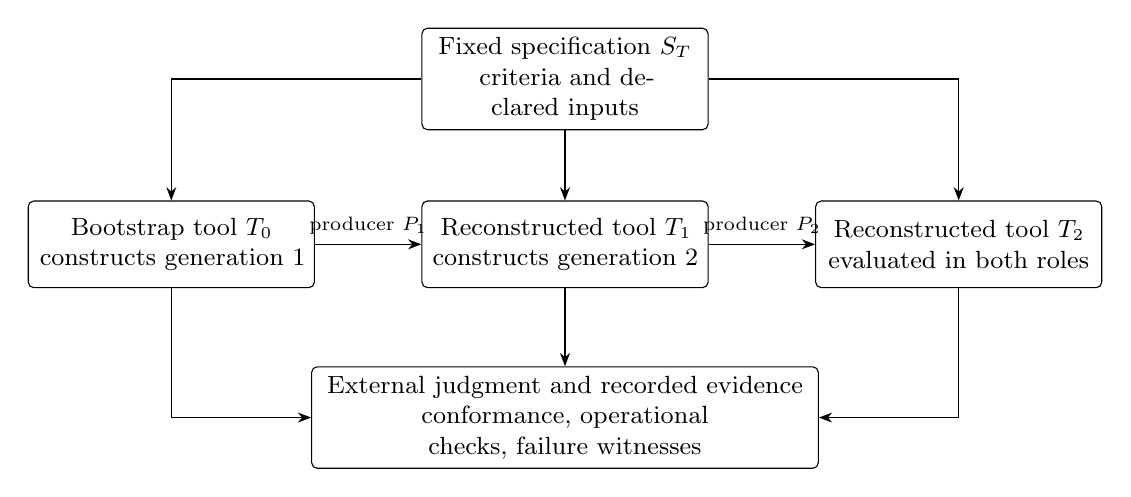
\begin{tikzpicture}[>=Stealth,box/.style={draw,rounded corners=2pt,align=center,font=\small,minimum height=11mm,text width=3.4cm},lab/.style={font=\scriptsize,align=center}]
\node[box] (s) at (0,2.1) {Fixed specification $S_T$\\criteria and declared inputs};
\node[box] (t0) at (-5,0) {Bootstrap tool $T_0$\\constructs generation 1};
\node[box] (t1) at (0,0) {Reconstructed tool $T_1$\\constructs generation 2};
\node[box] (t2) at (5,0) {Reconstructed tool $T_2$\\evaluated in both roles};
\node[box,text width=6.2cm] (j) at (0,-2.2) {External judgment and recorded evidence\\conformance, operational checks, failure witnesses};
\draw[->] (t0)--node[above,lab]{producer $P_1$}(t1);
\draw[->] (t1)--node[above,lab]{producer $P_2$}(t2);
\draw[->] (s)--(t1);
\draw[->] (s.west)-| (t0.north);
\draw[->] (s.east)-| (t2.north);
\draw[->] (t0.south)|-(j.west);
\draw[->] (t1.south)--(j.north);
\draw[->] (t2.south)|-(j.east);
\end{tikzpicture}
\caption{Self-hosting reconstruction preserves a specification across changes in implementation and in the tool responsible for construction. Producers and runtime infrastructure remain explicit external dependencies. Each generated tool is tested as a candidate and in operation; the successor is not accepted solely on its parent's assertion. A change to the specification starts a new experimental series.}
\label{fig:succession}
\end{figure*}

\subsection{Execute the successor step}
Let $S_T$ specify the reconstruction tool itself. The initial step is
\begin{equation}
 (T_1,\tau_1)=R_{T_0}(S_T,P_1;e,b).
\end{equation}
After $T_1$ passes object- and operator-role checks, transfer reconstruction responsibility to it:
\begin{equation}
 (T_2,\tau_2)=R_{T_1}(S_T,P_2;e,b).
\end{equation}
The target identifier remains $\rho(S_T)$, but the implementation digests may differ. A second producer family can be used for $P_2$; this varies an experimental condition without establishing independence of failures. Figure~\ref{fig:succession} shows the separation between preserved specification, replaced tool, and external judgment.

Reconstructing a small component through $T_1$ is an initial operator test. Reconstructing the complete tool through $T_1$ is a stronger successor experiment. The two should be reported separately. In particular, a full generation-2 system that subsequently reconstructs a core component has not yet produced a full generation-3 system.

The invariant being tested is membership under one specification, not equality of source code. It is possible for every observed generation to preserve that invariant while differing internally. Conversely, a finite successful chain does not prove that all future producers or generations will preserve it. A universal closure result would require stronger assumptions and evidence than the observed executions supply.

\subsection{Record construction, transfer, and reconstruction separately}
Three observations make a result interpretable, and they are not interchangeable. First, record the original realization and its acceptance. Second, move the artifacts to another environment and re-run the checks; this separates portability from regeneration. Third, reconstruct from the declared view and evaluate the replacement. Each covers a gap the others leave. Copying artifacts locally says nothing about independent operation. Independent operation says nothing about whether the producer had access to the original.

For each run, retain the target identifier, implementation digest, producer configuration, visible inputs, tool version, runtime and platform information, resource limits, random seeds, all attempts, and exact verdicts. The dependency closure required to replay judgment must travel with the record, or be explicitly identified as an external requirement. A signed record attributes a claim to an operator; it does not independently verify the circumstances the operator attests to.

\section{Discovering and refining missing obligations}
\label{sec:obligations}
\subsection{The evaluator is a consumer}
The evaluator usually consumes the system it evaluates. Its scripts import a generated module, invoke a command, parse an output, or depend on a filesystem convention. Every one of those is a consumer requirement. If the local criteria leave such a requirement unstated, a conforming reconstruction can break the evaluator before the intended judgment even runs.

Let $U(J,I)$ denote the behaviors of candidate $I$ used by evaluator $J$. A practical review asks whether each required behavior in $U$ is covered by an interface contract and an executable check. Static analysis of imports, function calls, and command arguments can identify suspicious gaps, while dynamic reconstruction tests whether those gaps matter. Coverage of names alone is insufficient: a test may call an interface without exercising the case on which the evaluator depends.

This yields a useful distinction. A missing public obligation should usually strengthen the specification. An accidental dependency on a private implementation detail may instead require simplifying the evaluator. Reconstruction provides the witness; engineering judgment determines which side of the contract should change.

\subsection{Classify failures before changing the specification}
\label{sec:classify}
Not every unsuccessful run is specification discovery. Five cases need separating. A candidate that violates an existing check is an implementation failure. A valid system stopped by missing credentials is an infrastructure failure. An accepted implementation that breaks a justified consumer expectation is a specification omission. A check that rejects behavior the intended contract permits is an evaluator defect. And a declared time or memory overrun is a resource failure, which may in turn reveal a missing complexity requirement in the component criteria.

These categories can overlap, so the record should preserve the minimal reproducer, the candidate behavior, the expected behavior, and the experiment supporting the diagnosis. A repair should be tested both ways: it should reject the witnessed failure and accept a known intended behavior. This guards against replacing one omission with an incorrect restriction.

\subsection{Version the refinement}
For a deterministic evaluation under fixed conditions, adding an obligation $w$ conjunctively gives
\begin{equation}
 S'=S\land w \quad\Rightarrow\quad \mathcal{I}_{S'}\subseteq\mathcal{I}_{S}.
\end{equation}
The new specification receives a new identifier. Old runs remain evidence about $S$ and cannot silently become successes at $S'$. Corrections that relax or replace criteria are also legitimate, but do not satisfy this monotonicity relation automatically.

A campaign can alternate frozen reconstruction series with explicit revisions. Within a series, the target and success conditions remain unchanged; between series, an adopted witness changes the target. A declared stopping rule, such as several successful reconstructions across producer families and an independent replay, provides an operational milestone. It is not a proof that the specification has no further omissions.

\subsection{Measure sampled behavior separately from logical refinement}
\label{sec:sampled}
A genuinely stronger specification need not produce fewer observed divergences. Generated implementations are samples from a producer-dependent distribution $q(I\mid S,P)$. Changing $S$ changes two things at once: the admitted set, and the distribution of candidates actually drawn. So a new implementation can satisfy the added obligation and still reveal some other untested behavior.

External probes and downstream consumers therefore complement the acceptance gate. They can identify differences without initially turning those differences into requirements. Comparators may disagree for legitimate reasons, and a consumer may require behavior inappropriate for other consumers. Refinement must state whose requirements are being preserved.

Fixed examples have a further limitation: their accepted class can include a table of the observed answers. Generated properties and metamorphic relations make that strategy less effective, but finite randomized testing still supplies empirical evidence rather than complete semantics. Seeds and generator definitions belong in the experimental record.

One asymmetry decides whether a refinement's effect is visible at all. Divergences fall into classes: accepting input the reference rejects, rejecting input it accepts, returning a different value. Each producer family has a characteristic profile over those classes. Add an obligation against one class, and divergence in that class falls for every family. But a family's \emph{total} moves only in proportion to that class's share of its divergence.

The external pilot shows the consequence. Over-permissiveness was about half of one family's divergence and under a fifth of the other's. The refinement reduced that class in both families, and the total in only one (\artifact{research/external/jq/cross-family-finding.md}{decomposition}). A single aggregate over a single family can therefore show nothing where the refinement worked exactly as designed. Report the class decomposition, not the total.

\section{Prototype and empirical observations}
\label{sec:empirical}
\subsection{Implementation and evidence}
Reticuli implements the specification/implementation separation with content-derived roots, artifact transport, sandboxed judgment, and producer adapters. Its self-reconstruction harness builds components in dependency order using generated lower-layer code. Intermediate scaffold roots vary with their supplied inputs; the assembled tool is judged at a fixed system root.

The evidence analyzed here is the public snapshot \texttt{5318acaac34e}~\cite{repo}. It includes generated source trees, criteria, construction drivers, JSON results, and a dated trial ledger (\artifact{research/metrics/closure-ledger.md}{closure ledger}; \artifact{research/metrics/genome-map.md}{refinement register}; \artifact{research/metrics/freedom-register.md}{classified freedoms}). This paper synthesizes those artifacts; the producer calls and independent replay were not newly executed for manuscript preparation. The accompanying evidence index maps the following observations to exact files.

\subsection{Self-hosting reconstruction}
At target root prefix \texttt{900b6594}, the \artifact{research/metrics/closure-ledger.md}{ledger} records three qualifying runs: a Codex reconstruction, a Claude reconstruction, and a Codex-authored generation-2 reconstruction orchestrated by the Claude generation-1 kernel. Each qualifier's verdict is itself sealed as a claim whose gate re-executes the checks rather than restating them (\artifact{research/harness/closure/trial_claim.py}{builder}, \artifact{research/harness/closure/trialclaims}{sealed trials}). The final campaign reports 21 construction layers, full system acceptance, 104/104 held-out checks, bootstrap checks, and recursive operations for these qualifiers. They are selected successes at the final boundary, not a success-rate estimate over a fixed population of attempts.

The \artifact{research/harness/succession/run_grandchild.py}{generation-2 driver} loads the reconstructed kernel and packaging implementation to seal scaffolds, execute reconstruction, and confine gates. This establishes a concrete transfer of operational responsibility. The retained infrastructure includes the Python runtime, external model and producer adapter, experiment driver, decomposition metadata, and original-source scaffold inputs used in setup. Reconstructed lower-layer bytes are substituted into the producer rooms. Thus the reported source exclusion concerns those rooms; it does not mean that original artifacts have disappeared from the surrounding experiment.

The generated generation-2 system also passes recorded operator checks and reconstructs a core claim through its own interface. That result establishes a further component-level successor step. A full generation-3 reconstruction is not established by the core-step record. The ledger's outside-machine condition remains pending; an archived re-execution JSON contains passing measurements but does not, by itself, establish an independent operator. The protocol an external operator would follow, and the receipt it produces, are specified in advance (\artifact{research/harness/closure/outside.md}{protocol}). Table~\ref{tab:roles} summarizes the scope of the evidence.

\begin{table}[t]
\centering\small
\begin{tabular}{@{}p{0.44\columnwidth}p{0.50\columnwidth}@{}}
\toprule
Experiment & Archived observation\\
\midrule
Object-role conformance & Two families qualify at one final boundary.\\[3pt]
Operator-role checks & Generated tools audit, transport, and reconstruct.\\[3pt]
Full successor construction & Generation 1 orchestrates a complete generation 2.\\[3pt]
Further successor step & Generation 2 reconstructs a core component.\\[3pt]
Independent outside replay & Not established as complete in the closure ledger.\\
\bottomrule
\end{tabular}
\caption{Different claims require different evidence. Full self-hosting construction, component-level recursion, and independent replay are reported separately.}
\label{tab:roles}
\end{table}

\subsection{Failures that informed the method}
Three findings illustrate why the role distinction and composition tests matter. First, generated component records could pass local checks yet fail a later deep audit because the writer emitted a lean record while the reader expected additional fields. Testing the writer--reader round trip encoded the missing contract directly.

Second, a generated execution layer could pass simple confinement tests but deny an operating-system service required by the complete acceptance suite. The candidate passed as content under the existing evaluator and failed as the evaluator. A subsequent criterion exercised legitimate execution as well as prohibited behavior. This is an operator-role requirement that ordinary substitution under a reference harness can miss.

Third, a generated dependency traversal repeatedly walked shared ancestry, producing excessive growth and exceeding the declared system window. The repair introduced incremental-construction and growth constraints. Functional answers on small inputs had not captured the operational requirement to complete construction at the intended scale.

These examples support the method's use of integration witnesses, operator tests, and explicit resource envelopes. They do not imply that every adopted repair generalizes beyond the witnessed contract. The campaign also records withdrawn diagnoses, and boundary changes that reset earlier success counts. Two registers keep this legible. One lists each adopted obligation, the refusal that selected it, and the later reconstructions it did or did not steer (\artifact{research/metrics/genome-map.md}{refinement register}). The other lists the behaviors left deliberately unconstrained, with reasons (\artifact{research/metrics/freedom-register.md}{companion register}). The second list matters as much as the first. A method that only adds obligations converges on one implementation and stops describing a class.

\subsection{Supporting substitution experiments}
A deliberately underspecified key--value parser provides a compact consumer test. Six model-produced implementations, three from each of two families, passed the parser gate; all six failed a consumer that required numeric coercion and last-key-wins behavior (\artifact{research/harness/substitution}{harness}). Six new reconstructions from a boundary containing those obligations passed the consumer. This demonstrates a specific omission and repair, while showing that cross-family agreement can preserve the same unsuitable interpretation.

An external jq evaluation-core pilot provides a complementary boundary-design example. A first reconstruction passed all 465 examples by implementing a lookup table --- its own header states that it is \emph{not} a general evaluator (\artifact{research/external/jq/evidence/sample1-the-lookup-table.py}{generated source}; \artifact{research/external/jq/generation-1.md}{analysis}; \artifact{research/external/jq/preregistration.md}{preregistration}). It agreed with reference jq on 587 of 1,395 novel probes and errored on the remaining 808. Subsequent boundaries added generated properties and error-handling laws. The result motivates richer executable criteria, rather than treating an example corpus as a complete description of an evaluator.

The same campaign illustrates the discipline of Section~\ref{sec:sampled}, including a withdrawal. We first claimed that one refinement cut aggregate divergence by 25\%. Our own preregistered control refuted it. Fresh reconstructions at an \emph{unchanged} boundary came back no lower than before, and the spread within a single boundary exceeded the effect we had reported (\artifact{research/external/jq/generation-4-control-CORRECTION.md}{control and withdrawal}). The lesson is about the metric. An aggregate count discards the pairing between a probe before and after refinement, and the pairing is where the information sits.

Paired per probe, the archived samples show a clear asymmetry. Fifteen behaviors diverged consistently before the refinement and in no sample after it. One went the other way. That is an exact one-tailed binomial $p\approx 2.6\times 10^{-4}$, and the closed behaviors trace by name to the obligations that closed them. The asymmetry also grew as samples accumulated, from 10:1 to 15:1 (\artifact{research/external/jq/rate-metric-findings.md}{analysis}, \artifact{research/external/jq/rate_metric.py}{instrument}). Sampling noise weakens with more data; a real effect sharpens.

We still treat the result as exploratory. The probes are correlated. The analysis was adaptive. The comparison covers one producer family at one refinement. And the self-hosting result does not rest on it.

\subsection{Byproduct: divergences in the compared implementations}
Writing executable criteria against a real target means deciding what the target refuses. That decision has to be checked against the target, not assumed. Checking it surfaced behavior that none of the compared implementations documents. Three examples follow. Each is reproducible with one command and recorded with its transcript (\artifact{research/external/jq/ecosystem-findings.md}{transcripts}).

\begin{itemize}\itemsep1pt\parskip0pt
\item \texttt{reverse} applied to \texttt{0} returns the empty array in the reference and raises in both reimplementations. The reference defines \texttt{reverse} through \texttt{length}. A zero-length input indexes nothing, so the type error never fires. \texttt{reverse} of \texttt{5} raises as expected.
\item \texttt{range("a")} raises in the reference and in one reimplementation. In the other it does not terminate.
\item A string repeated $10^9$ times returns promptly in both reimplementations. In the reference it does not terminate.
\end{itemize}

None of this is central to the method's claims. We report it for two reasons. A reader can check these in seconds, which is otherwise hard for the results in this paper. And they show that authoring obligations is itself a source of findings about deployed software, not merely bookkeeping.

The same checking step also rejected three obligations we had drafted ourselves. The reference's refusals turned out to be value-dependent rather than type-dependent, so the rules we had written were false. That is the discipline of Section~\ref{sec:classify} applied to our own proposals.

\section{Relationship to prior work}
\paragraph{Compiler bootstrapping and trust.} Self-hosting has a long history in compiler construction. Thompson's account of compiler-borne attacks shows that a tool's ability to reproduce itself cannot establish its trustworthiness~\cite{thompson}. Diverse double-compiling uses a trusted diverse compiler to test correspondence between source and executable under stated assumptions~\cite{wheeler}. The method here asks a different question: whether fresh implementation bytes can be constructed from executable requirements and then operate as the reconstruction tool. It does not eliminate the trusted runtime or establish source--binary correspondence.

\paragraph{Verified self-hosting.} CakeML connects an executable compiler to a formal semantics and bootstraps a verified compiler within a theorem prover~\cite{cakeml}. This supplies stronger semantic guarantees than passing a finite test suite. Our approach occupies an empirical setting in which the specification is executable but incomplete. Its purpose is to identify and test the operational conditions for successive reconstruction, including omissions revealed by regenerated implementations.

\paragraph{Synthesis and refinement.} Counterexample-guided inductive synthesis alternates candidate generation and validation against a specification~\cite{solar}. We use a related experimental loop but distinguish candidate refinement under a fixed specification from revision of the specification itself. A downstream failure may justify a new requirement; adopting it changes the target rather than retroactively disqualifying the earlier experiment as a generation failure. Language-model evaluation by executable tests, exemplified by HumanEval~\cite{humaneval}, provides a practical generator-and-gate setting for this distinction.

\paragraph{Recovering implicit obligations.} Dynamic invariant inference observes executions and proposes properties the program appears to maintain, as in Daikon~\cite{daikon}. That line of work and this one share a goal --- making implicit requirements explicit --- and differ in the probe. Invariant inference generalizes from executions of the \emph{existing} implementation; reconstruction generates \emph{new} implementations and treats their disagreements as evidence about the specification. The two are complementary: inferred invariants are candidate obligations, and a reconstruction that violates one indicates either a missing obligation or an overgeneralized inference.

\paragraph{Testing and diversity.} Differential testing exposes disagreements among implementations, as demonstrated by Csmith~\cite{csmith}. QuickCheck and metamorphic testing provide established ways to express properties over generated inputs and relations between executions~\cite{quickcheck,metamorphic}. These techniques can strengthen reconstruction criteria or remain external probes. The observation that separate producers can fail alike also follows a longstanding concern in multiversion programming, whose design~\cite{avizienis} and empirical refutation of the independence assumption~\cite{knight} both predate this setting; distinct source code is not evidence of independent errors. What changes here is cost: generating a version is now cheap enough to run the experiment many times, which was the practical obstacle rather than the conceptual one.

\paragraph{Reproducible builds.} Reproducible builds aim to recover identical artifacts from the same source and build conditions~\cite{builds}, and bootstrappable-build efforts additionally minimize the trusted binary seed~\cite{bootstrappable}. Reconstruction preserves a declared acceptance target while permitting different source. Both are useful: reproducible builds help validate artifact provenance, while reconstruction tests whether the preserved specification supports replacement and continued operation. Neither property subsumes the other.

\section{Discussion}
The main consequence of self-hosting reconstruction is methodological. It makes the evaluator's own requirements observable through replacement. A fixed implementation can satisfy an implicit interface for years; a reconstructed implementation may satisfy the declared interface while exposing that hidden dependence immediately. The resulting witness can improve the specification, remove an accidental evaluator dependency, or clarify the environment in which the claim holds.

A successful chain also suggests a useful distinction between preserving software and preserving the capacity to realize it. Source archives preserve a particular implementation. An executable specification plus a functioning reconstruction tool and producer preserves an experimentally demonstrated route to another accepted implementation. That route remains conditional on the available infrastructure, resources, and strength of the criteria.

The present evidence has clear limits, and the first is structural. One person authored the criteria and designed the method. Those criteria were then revised repeatedly in response to how the two producer families behaved. Specification and probe population thus co-evolved. That is the right way to \emph{develop} a boundary, and a confound when \emph{measuring} one. A boundary authored independently of the producers would be a stronger test; this campaign does not provide one.

Other limits follow. The main case is the reconstruction instrument itself. The parser is deliberately constructed. The jq pilot covers a restricted interface. Producer families may share training material and conventions. Held-out tests repeatedly consulted across a development campaign provide regression evidence but should not be treated as an untouched final evaluation set. Exact costs and success rates require accounting for retries, subscription use, and failed series, not only final qualifiers.

A stronger evaluation would freeze the target, tool versions, producer configurations, budgets, and primary outcomes before a balanced series of attempts. Independent operators would repeat judgment on transferred artifacts. Future work should measure how often full successors remain operational across generations, which interfaces account for failures, and how results change when producers or environments are varied. Specification revisions should be evaluated in a separate series with fresh probes and appropriate treatment of shared failure causes.

Self-hosting alone is not improvement. Improvement requires a separately declared objective, such as lower reconstruction cost, fewer justified consumer failures, or wider environment support at unchanged obligations. Successive construction and specification repair provide a way to study such objectives; they do not establish autonomous or unbounded improvement.

\section{Conclusion}
Executable specifications can serve as reconstruction targets whose identity survives replacement of implementation bytes. Applying this principle to the reconstruction tool creates a self-hosting experiment: each generated system must satisfy the target and carry out the work needed to produce a successor. Layered construction, separate object- and operator-role tests, explicit bootstrap dependencies, and versioned repairs make that experiment interpretable. The prototype records a finite instance of full successor construction and concrete failures that reveal missing obligations. Together, these results support self-hosting reconstruction as a practical method for investigating software replaceability and developing executable specifications.

\balance
\section*{Artifact availability}
The case-study snapshot is \texttt{5318acaac34ef99eeba9ff064a995a6313cc70ec} in the public Reticuli repository~\cite{repo}. The accompanying source package provides an evidence index, reproduction notes, and a read-only script for archived numerical summaries. No new producer runs or independent external replay were performed for this manuscript.

One data-management disclosure. Reconstructed implementations are destroyed after measurement by design. Separately, an early probe run wrote its output to a path that a later run reused, overwriting the first generation's probe-level records. Only that generation's summary and its generated source survived in the archive.

The loss was recoverable. Probe inputs are generated from fixed seeds, so we regenerated the records exactly from the preserved source: 587 agreements and 808 refusals over 1,395 probes, matching the figures recorded at the time. The regenerated file is included, and a reader can repeat the regeneration with the archived prober and source. No other number in this paper depends on a file that was overwritten.

\begin{thebibliography}{15}\small
\bibitem{repo} R. Zamora-Resendiz. \emph{Reticuli}. Repository snapshot, October 12, 2026. \url{https://github.com/rz4/reticuli/tree/5318acaac34ef99eeba9ff064a995a6313cc70ec}.
\bibitem{thompson} K. Thompson. Reflections on trusting trust. \emph{Communications of the ACM}, 27(8):761--763, 1984. doi:10.1145/358198.358210.
\bibitem{wheeler} D. A. Wheeler. \emph{Fully Countering Trusting Trust through Diverse Double-Compiling}. Ph.D. dissertation, George Mason University, 2009. \url{https://arxiv.org/abs/1004.5534}.
\bibitem{cakeml} R. Kumar, M. O. Myreen, M. Norrish, and S. Owens. CakeML: A verified implementation of ML. \emph{POPL}, 2014. doi:10.1145/2535838.2535841.
\bibitem{solar} A. Solar-Lezama. \emph{Program Synthesis by Sketching}. Ph.D. thesis, University of California, Berkeley, 2008. \url{https://www2.eecs.berkeley.edu/Pubs/TechRpts/2008/EECS-2008-177.html}.
\bibitem{humaneval} M. Chen et al. Evaluating large language models trained on code. 2021. \url{https://arxiv.org/abs/2107.03374}.
\bibitem{csmith} X. Yang, Y. Chen, E. Eide, and J. Regehr. Finding and understanding bugs in C compilers. \emph{PLDI}, 2011. doi:10.1145/1993498.1993532.
\bibitem{quickcheck} K. Claessen and J. Hughes. QuickCheck: A lightweight tool for random testing of Haskell programs. \emph{ICFP}, pp. 268--279, 2000. doi:10.1145/351240.351266.
\bibitem{metamorphic} T. Y. Chen, S. C. Cheung, and S. M. Yiu. \emph{Metamorphic Testing: A New Approach for Generating Next Test Cases}. Technical Report HKUST-CS98-01, 1998. \url{https://arxiv.org/abs/2002.12543}.
\bibitem{knight} J. C. Knight and N. G. Leveson. An experimental evaluation of the assumption of independence in multiversion programming. \emph{IEEE Transactions on Software Engineering}, SE-12(1):96--109, 1986. doi:10.1109/TSE.1986.6312924.
\bibitem{daikon} M. D. Ernst, J. H. Perkins, P. J. Guo, S. McCamant, C. Pacheco, M. S. Tschantz, and C. Xiao. The Daikon system for dynamic detection of likely invariants. \emph{Science of Computer Programming}, 69(1--3):35--45, 2007. doi:10.1016/j.scico.2007.01.015.
\bibitem{avizienis} A. Avi\v{z}ienis. The N-version approach to fault-tolerant software. \emph{IEEE Transactions on Software Engineering}, SE-11(12):1491--1501, 1985. doi:10.1109/TSE.1985.231893.
\bibitem{bootstrappable} J. Janneke, L. Courtès, et al. Bootstrappable builds and the full-source bootstrap. \url{https://bootstrappable.org/}, accessed October 2026.
\bibitem{builds} C. Lamb and S. Zacchiroli. Reproducible builds: Increasing the integrity of software supply chains. 2021. \url{https://arxiv.org/abs/2104.06020}.
\end{thebibliography}
\end{document}
